\documentclass[twoside,10pt,a4paper]{article}
\usepackage[utf8]{inputenc}
\usepackage[english]{babel}
\usepackage{amsmath}
\usepackage{amsfonts}
\usepackage{amssymb}
\usepackage{graphicx}

\usepackage[left=2cm,right=2cm,top=2cm,bottom=3cm]{geometry}
\usepackage{fancyvrb}
\usepackage{listings}
\usepackage{xparse}
\usepackage{tikz} % ajout de dessins LaTeX
\usepackage{graphicx}
\usepackage{float}  % alignement des figures
\usepackage{fancyhdr}
\usepackage{enumitem}
\usepackage{verbatim}
\usepackage{xcolor}
\usepackage{mathtools}
\usepackage{cancel}


\usepackage{caption}
\usepackage{subcaption}

\pagestyle{fancy} %fancyhdr
	\fancyhf{} %fancyhdr
	\renewcommand{\sectionmark}[1]{\markboth{#1}{}}
	\fancyhead[R]{Exercice Set 1 - Questions} %INSERT TITLE HERE FOR fancyhdr
	\fancyhead[L]{\nouppercase{\leftmark}} %fancyhdr
	\cfoot{\thepage} %fancyhdr
	\setlength{\headheight}{35pt}
	\setlength{\parindent}{0pt}
	
	\definecolor{MyBlue}{HTML}{4A90E2}
	\definecolor{MyRed}{HTML}{D0021B}
	\definecolor{MyGreen}{HTML}{7ED321} % Same color use in Mathcha

\begin{titlepage}
\title{\huge \textbf{Nonlinear Dynamics and Chaos I \\ \Large  Exercice Set 1 - Questions}}	%TITLE
\author{ }		%AUTHOR
\date{ }	%DATE

\end{titlepage}


\begin{document}

\maketitle

\section*{Question 1}
Many important properties of nonlinear dynamical systems follow from Gronwall's inequality. Assume that two positive, continuous scalar functions $u(t)$ and $v(t)$ satisfy the condition
\begin{equation*}
	u(t) \leq C + \int_{t_0}^t u(\tau)v(\tau) \, \text{d}\tau
\end{equation*}
for some constant $C \geq 0$ and for all $t \geq t_0$. Then Gronwall's inequality asserts that
\begin{equation*}
u(t) \leq Ce^{\int_{t_0}^t v(\tau) \, \text{d}\tau} 
\end{equation*}
for all $t \geq t_0$. The significance of this result is that it gives a $u(t)$-independent upper bound on the growth of $u(t)$. Using Gronwall's inequality, give an upper bound on how fast the solutions of a nonlinear ODE can separate from each other in time. In particular, show that for an ODE of the form
\begin{equation*}
	\dot{x} = f(x,t), \qquad x \in \mathbb{R}^n,
\end{equation*}
and for two solutions starting from the initial conditions $x_0$ and $\hat{x}_0$ at time $t_0$, we have
\begin{equation*}
	|x(t, x_0) - x(t, \hat{x}_0)| \leq |x_0 - \hat{x}_0|e^{L(t - t_0)},
\end{equation*}
where $L$ is a Lipschitz constant for the function $f$ over a domain containing the trajectories of the system over the time interval $[t_0, t]$.

\textit{Hint}: Substitute both solutions into the ODE, integrate the resulting two equations from $t_0$ to $t$, and estimate their normed difference.

\section*{Question 2}
Consider a pendulum that strikes an inclined wall repeatedly, as shown in Fig. \ref{Q01D01} below. Using the phase portrait of the pendulum discussed in class, sketch the trajectories in the phase space of this impact dynamical system for positive and negative values of the angle $\alpha$, when

\begin{enumerate}[label=(\roman*)]
	\item there us no loss of energy at impact
	\item the coefficient of restitution is 0.5.
\end{enumerate}
Identify the asymptotic behavior of the pendulum in each case.

\begin{figure}[H]
	\centering
	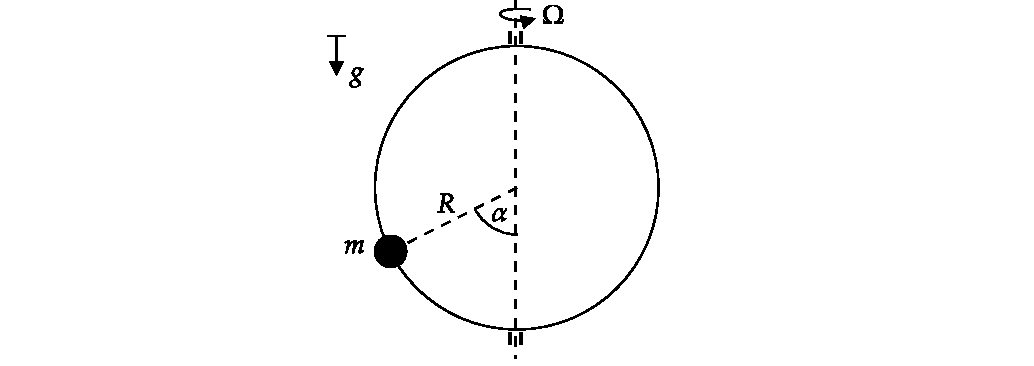
\includegraphics[scale=0.9]{Graphics/Q01D01.pdf}
	\caption{Pendulum attached to the inclined wall.}
	\label{Q01D01}
\end{figure}

\textit{Hint}: During impact, the pre-impact velocity of the pendulum is assumed to jump instantaneously to its post-impact value, while the pendulum's position remains the same.

\section*{Question 3}
Consider the non-dimensionalized, force-damped pendulum equation
\begin{equation*}
	\ddot{x} + k\dot{x} + \sin(x) = a\sin(t),
\end{equation*}
where $k \geq 0$ is the damping coefficient and $a \geq 0$ is the forcing amplitude.

\begin{enumerate}[label=(\alph*)]
	\item For vanishing damping and forcing $(a=k=0)$, compute and plot numerically the FTLE field for this system over a $100 \times 100$ grid of initial conditions, covering the square $[- \pi, \pi] \times [-\pi, \pi]$ in the phase space of the pendulum. Perform the computation for long enough times so that the FTLE plot fully reveals the separatrices of the system, as we discussed in class for the undamped pendulum.
	\item To explore the fate of these separatrices under mild damping and forcing, repeat the same FTLE computations for $a = 0.5$ and $k = 0.1$. Discuss domains of attractions and their boundaries based on the results.
\end{enumerate}

\textit{Hint}: Consider using MATLAB’s ODE45 routine for trajectory integration. To this end, you need to assemble all initial grid points into a single long vector, and pass that vector on to ODE45 as an initial condition. You will then need to define an appropriate extended ODE, whose right-hand side will be called by ODE45 to produce an advected image of the extended initial condition vector. Subsequently, you will need to convert the elements of this advected vector back into advected grid positions.
Alternatively, you could write your own 4-point Runge-Kutta solver to track trajectories simultaneously on the full grid of initial conditions (see the algorithm discussed in class).

\section*{Question 4}
Which figure describes the phase portrait of the following dynamical system ?
\begin{equation*}
	\ddot{x} = x(1 - x)
\end{equation*}

\begin{enumerate}[label=(\alph*)]
	\item  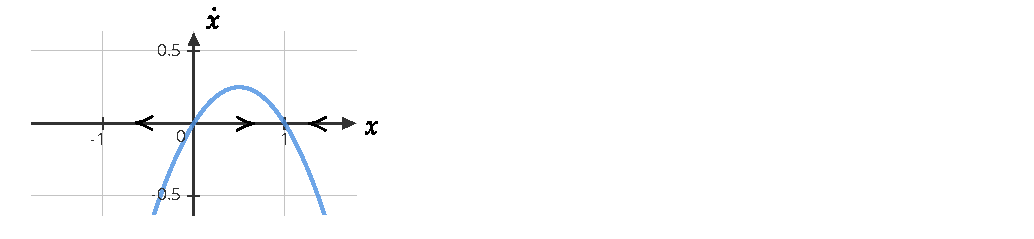
\includegraphics[scale=0.8]{Graphics/MCQ1_figures/Q02D01.pdf}
	\item  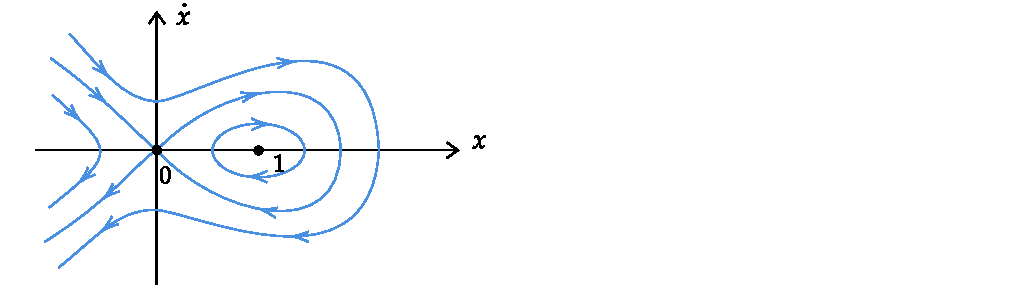
\includegraphics[scale=0.8]{Graphics/MCQ1_figures/Q02D02.pdf}
	\item  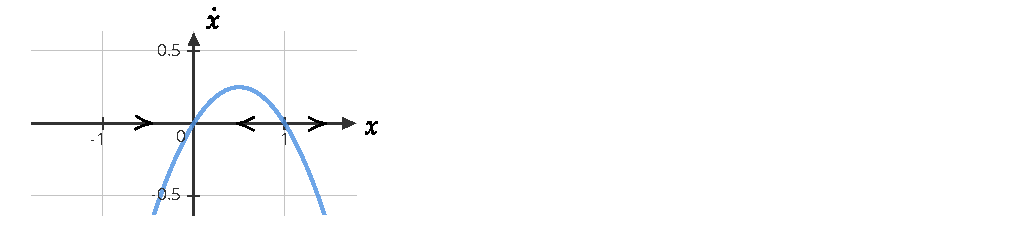
\includegraphics[scale=0.8]{Graphics/MCQ1_figures/Q02D03.pdf}
	\item  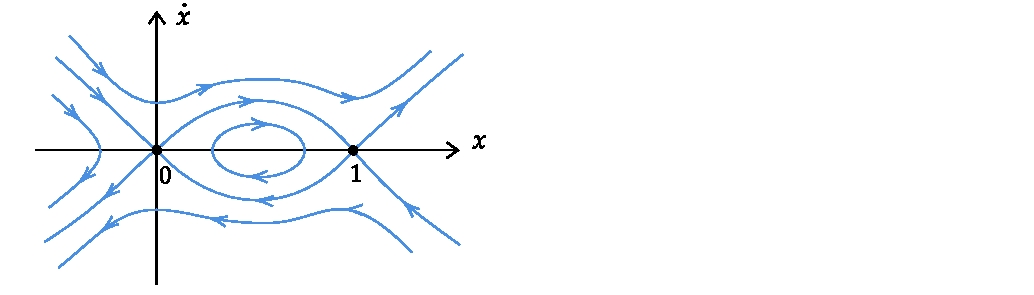
\includegraphics[scale=0.8]{Graphics/MCQ1_figures/Q02D04.pdf}
\end{enumerate}

\section*{Question 5}
Consider the following dynamical system with the solutions $x(t; t_0, x_0)$. For which system does the following estimate fail for any constant $C \geq 0$.
\begin{equation*}
	||x(t; t_0, x_0) - x(t; t_0, \tilde{x}_0) || \leq ||x - \tilde{x}_0||\,e^{C(t-t_0)}, \quad \forall t \geq t_0, \quad x_0, \tilde{x}_0 \geq 0
\end{equation*}

\begin{enumerate}[label=(\alph*)]
	\item $ \dot{x} = \sin(x) $
	\item $ \dot{x} = x^2 $
	\item $ \dot{x} = 100x $
	\item $ \dot{x} = e^{-x} $
\end{enumerate}

\section*{Question 6}
Which figure describes the phase portrait of the dynamical system
\begin{equation*}
	\ddot{x} + 2\dot{x} + \sin(x) = 0
\end{equation*}
near the equilibrium point $x = 0, \; \dot{x} = 0$?

\begin{enumerate}[label=(\alph*)]
	\item 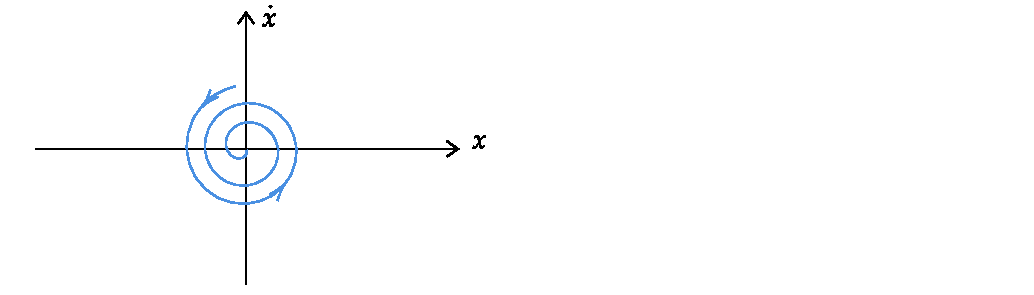
\includegraphics[scale=0.8]{Graphics/MCQ1_figures/Q08D01.pdf}
	\item 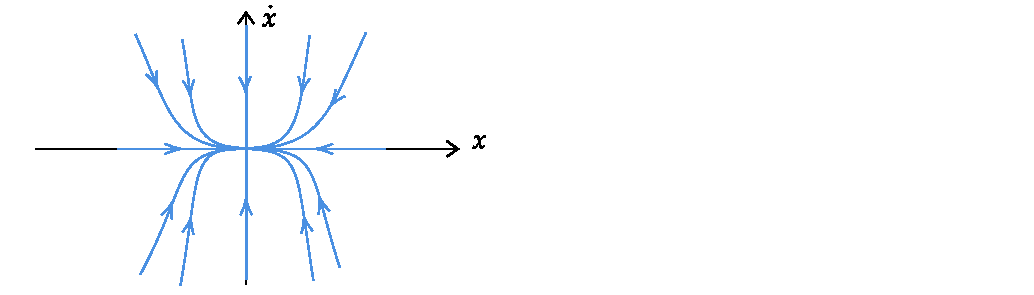
\includegraphics[scale=0.8]{Graphics/MCQ1_figures/Q08D02.pdf}
	\item 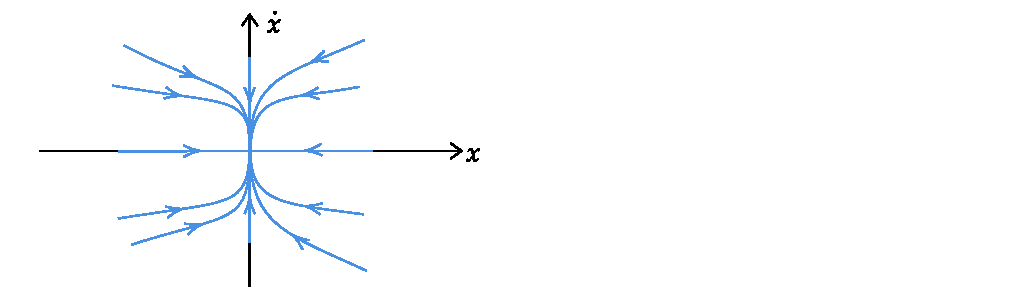
\includegraphics[scale=0.8]{Graphics/MCQ1_figures/Q08D03.pdf}
	\item 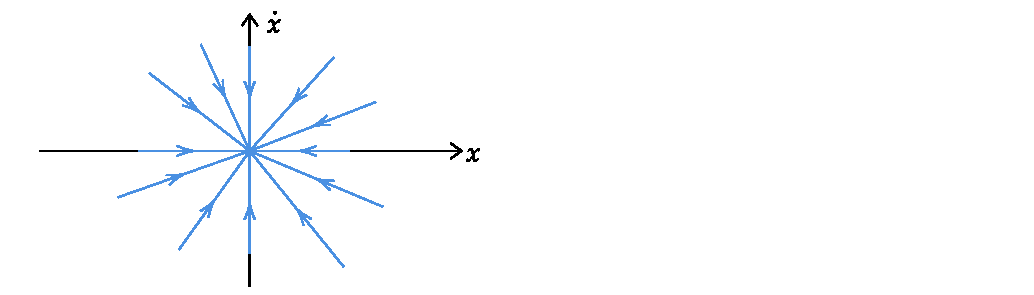
\includegraphics[scale=0.8]{Graphics/MCQ1_figures/Q08D04.pdf}
\end{enumerate}

\section*{Question 7}
Consider the 1D map
\begin{equation*}
	x_{n+1} = x_n^2(1 - x_n^2)
\end{equation*}
Which relation is the correct linearization around the fixed point $x = 0$?

\begin{enumerate}[label=(\alph*)]
	\item $ y_{n+1} = y_n(1 - y_n) $
	\item $ y_{n+1} = y_n(1 - y_n^2) $
	\item $ y_{n+1} = 0 $
	\item $ y_{n+1} = y_n $
\end{enumerate}

\end{document}